\chapter{Features, Scenarios, Stories}

\section{3 - Ottobre}
Which factor drive the design of SW products?
\begin{itemize}
    \item {\color{gray}Inspiration}
    \item Business/consumer needs not met by existing products
    \item Dissatisfaction with existing products
    \item Technical changes making new product types possible
\end{itemize}

Product-based software engineering needs less \textit{requirements documentation} than project-based SE, 
since the requirements are not set by customers and it is allowed for them to change.
The focus is instead on \textbf{features} (fragments of functionality); 
to understand which features are needed, we must first understand which may be \textbf{potential users}, through interviews, surveys, informal user analysis and consultation.

\subsection*{Flow-chart}
User representations {---} \textbf{personas} {---} and natural language descriptions {---} \textbf{scenarios} and \textbf{stories} {---} help driving the identification of product \textbf{features}:
\begin{figure}[h]
    \centering
    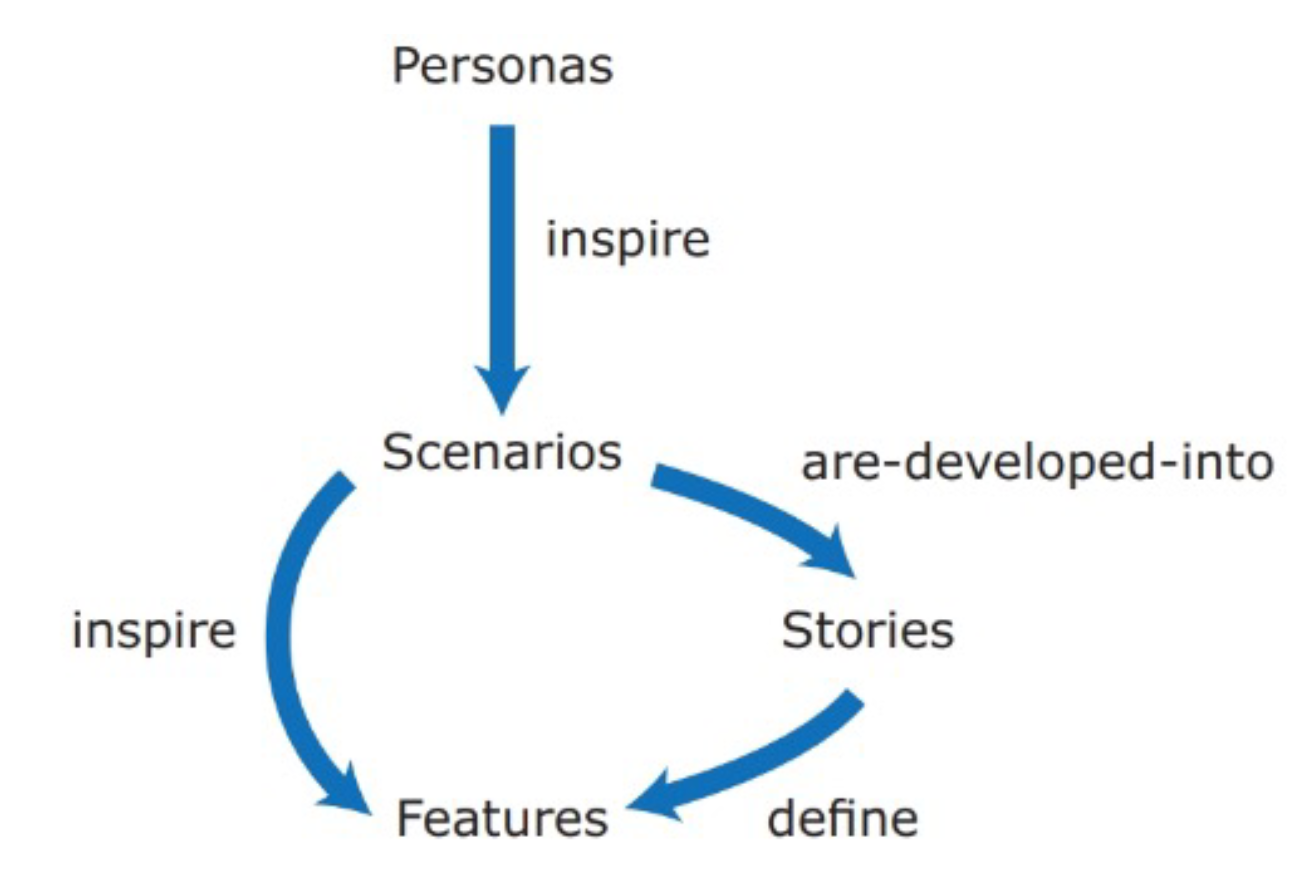
\includegraphics[width=0.5\textwidth]{images/features_flow.png}
    \caption{Features flowchart}
    \label{fig:features_flowchart}
\end{figure}

\section{Personas}
\textbf{Personas} represent the types of target users for our product.
Each personas should highlight which are \textit{background}, \textit{skills} and \textit{experience} of potential users.
Usually only a couple of personas (max 5) are needed to identify \textit{\textbf{key} product features}.
\nl

\begin{center}
\begin{tikzpicture}[main/.style = {draw, ellipse},node distance={3cm}] 
    \node[main] (P) {\textbf{PERSONA}};
    \node[main] (a) [align=center,above left=0.7cm and 2.5cm of P] {\textit{Personalization} \\ Include personal information \\ about the individual};
    \node[main] (b) [align=center, above right=0.7cm and 2.5cm of P] {\textit{Job-related} \\ Include details of \\ the individual's job};
    \node[main] (c) [align=center, below right= 0.7cm and 2.5cm of P] {\textit{Relevance} \\ Include details of their \\ interest in the product};
    \node[main] (d) [align=center, below left=0.7cm and 2.5cm of P] {\textit{Education} \\ Include details of their \\ education and experience};

    \draw[->] (P) -- (a);
    \draw[->] (P) -- (b);
    \draw[->] (P) -- (c);
    \draw[->] (P) -- (d);
\end{tikzpicture}
\end{center}

There are conflicting opinions about whether personas should include \textit{photos} or not.\\
Photos may be misleading, since \textit{"personas are not about how users look, but what they do"} (Steve Cable).
\textit{"Detailed personas encouraged the team to assume that demographic information drove motivations"} (Sara Wachter-Boettcher).

\section{Scenarios}
Having defined personas, to discover product features, it would aid to define \textit{user interactions} with the product:
a \textbf{scenario} is a narrative written from \textit{user's perspective} describing a situation in which a user is using our product's features to do something she wants to do.\\
Scenarios are \textbf{not} \textit{specifications}!
They lack details and may be incomplete.

\begin{center}
\begin{tikzpicture}[main/.style = {draw, ellipse},node distance={3cm}] 
    \node[main] (P) {\textbf{SCENARIO}};
    \node[main] (a) [align=center, above left=1cm and 2.5cm of P] {Scenario name};
    \node[main] (b) [align=center, left=1cm of P] {Overall objective};
    \node[main] (c) [align=center, below left=1cm and 2.5cm of P] {What's involved in \\ reaching the objective};
    \node[main] (d) [align=center, above right=1cm and 2.5cm of P] {Personas of actors \\ involved};
    \node[main] (e) [align=center, right=1cm and 1cm of P] {Problems that can't be \\ addressed by existing system};
    \node[main] (f) [align=center, below right=1cm and 2.5cm of P] {Possible ways that the problem \\ could be tackled};

    \draw[->] (P) -- (a);
    \draw[->] (P) -- (b);
    \draw[->] (P) -- (c);
    \draw[->] (P) -- (d);
    \draw[->] (P) -- (e);
    \draw[->] (P) -- (f);
\end{tikzpicture}
\end{center}

A proper amount of scenarios usually is 3-4 for each persona, aiming to cover the persona's main responsabilities.
Each team member should create scenarios and discuss them with the rest of team and (possibly) users.

\section{User Stories}
\begin{table}[h]
    \centering
    \begin{tabular}{|cc|}
        \hline
        \textbf{As a} & \hspace{2.5cm} $<$role$>$\\
        \textbf{I want to} & \hspace{2.5cm} $<$do something$>$ \\
        \textbf{So that} & \hspace{2.5cm} $<$reason/values$>$ \\
        \hline
    \end{tabular}
    \caption{User Stories}
    \label{tab:my_label}
\end{table}

While \textbf{scenarios} are high-level stories of product use, \textbf{User stories} are more fine-grained narratives.
They allow to organize and chunk work into units which represent actual value to the customer, ultimately building software incrementally from the users perspective.
Longer stories can be split into shorter stories, and to eventually prioritize them.\\
These words should recall \textit{1. 3. 7. 10.} agile principles described in Section \ref{subsec:agile_principles}.\\
In fact, usually \textit{Scrum product backlog} is a set of \textit{user stories} sorted according to priority.

Even though it is possible to express all functionalities describe in a \textit{scenario} using \textit{user-stories},
scenarios can read more naturally, make stories understanding easier, and provide more context.

\section{Feature identification}
Our goal is to get a list of features that define our product, keeping in mind some \textbf{properties}:
\begin{itemize}
    \item \textbf{Independence} $\rightarrow$ a feat should not dfepend on how other system feats are implemented and should not be affected by the order of activation of other feats
    \item \textbf{Coherence} $\rightarrow$ feats should be linked to a single item of functionality.
    They should not do more than one thing and should never have side effects
    \item \textbf{Relevance} $\rightarrow$ systesm feats should reflect the way users normally carry out some task.
    They should not offer obscure functionality that is rarely required.
\end{itemize}

\begin{figure}
    \centering
    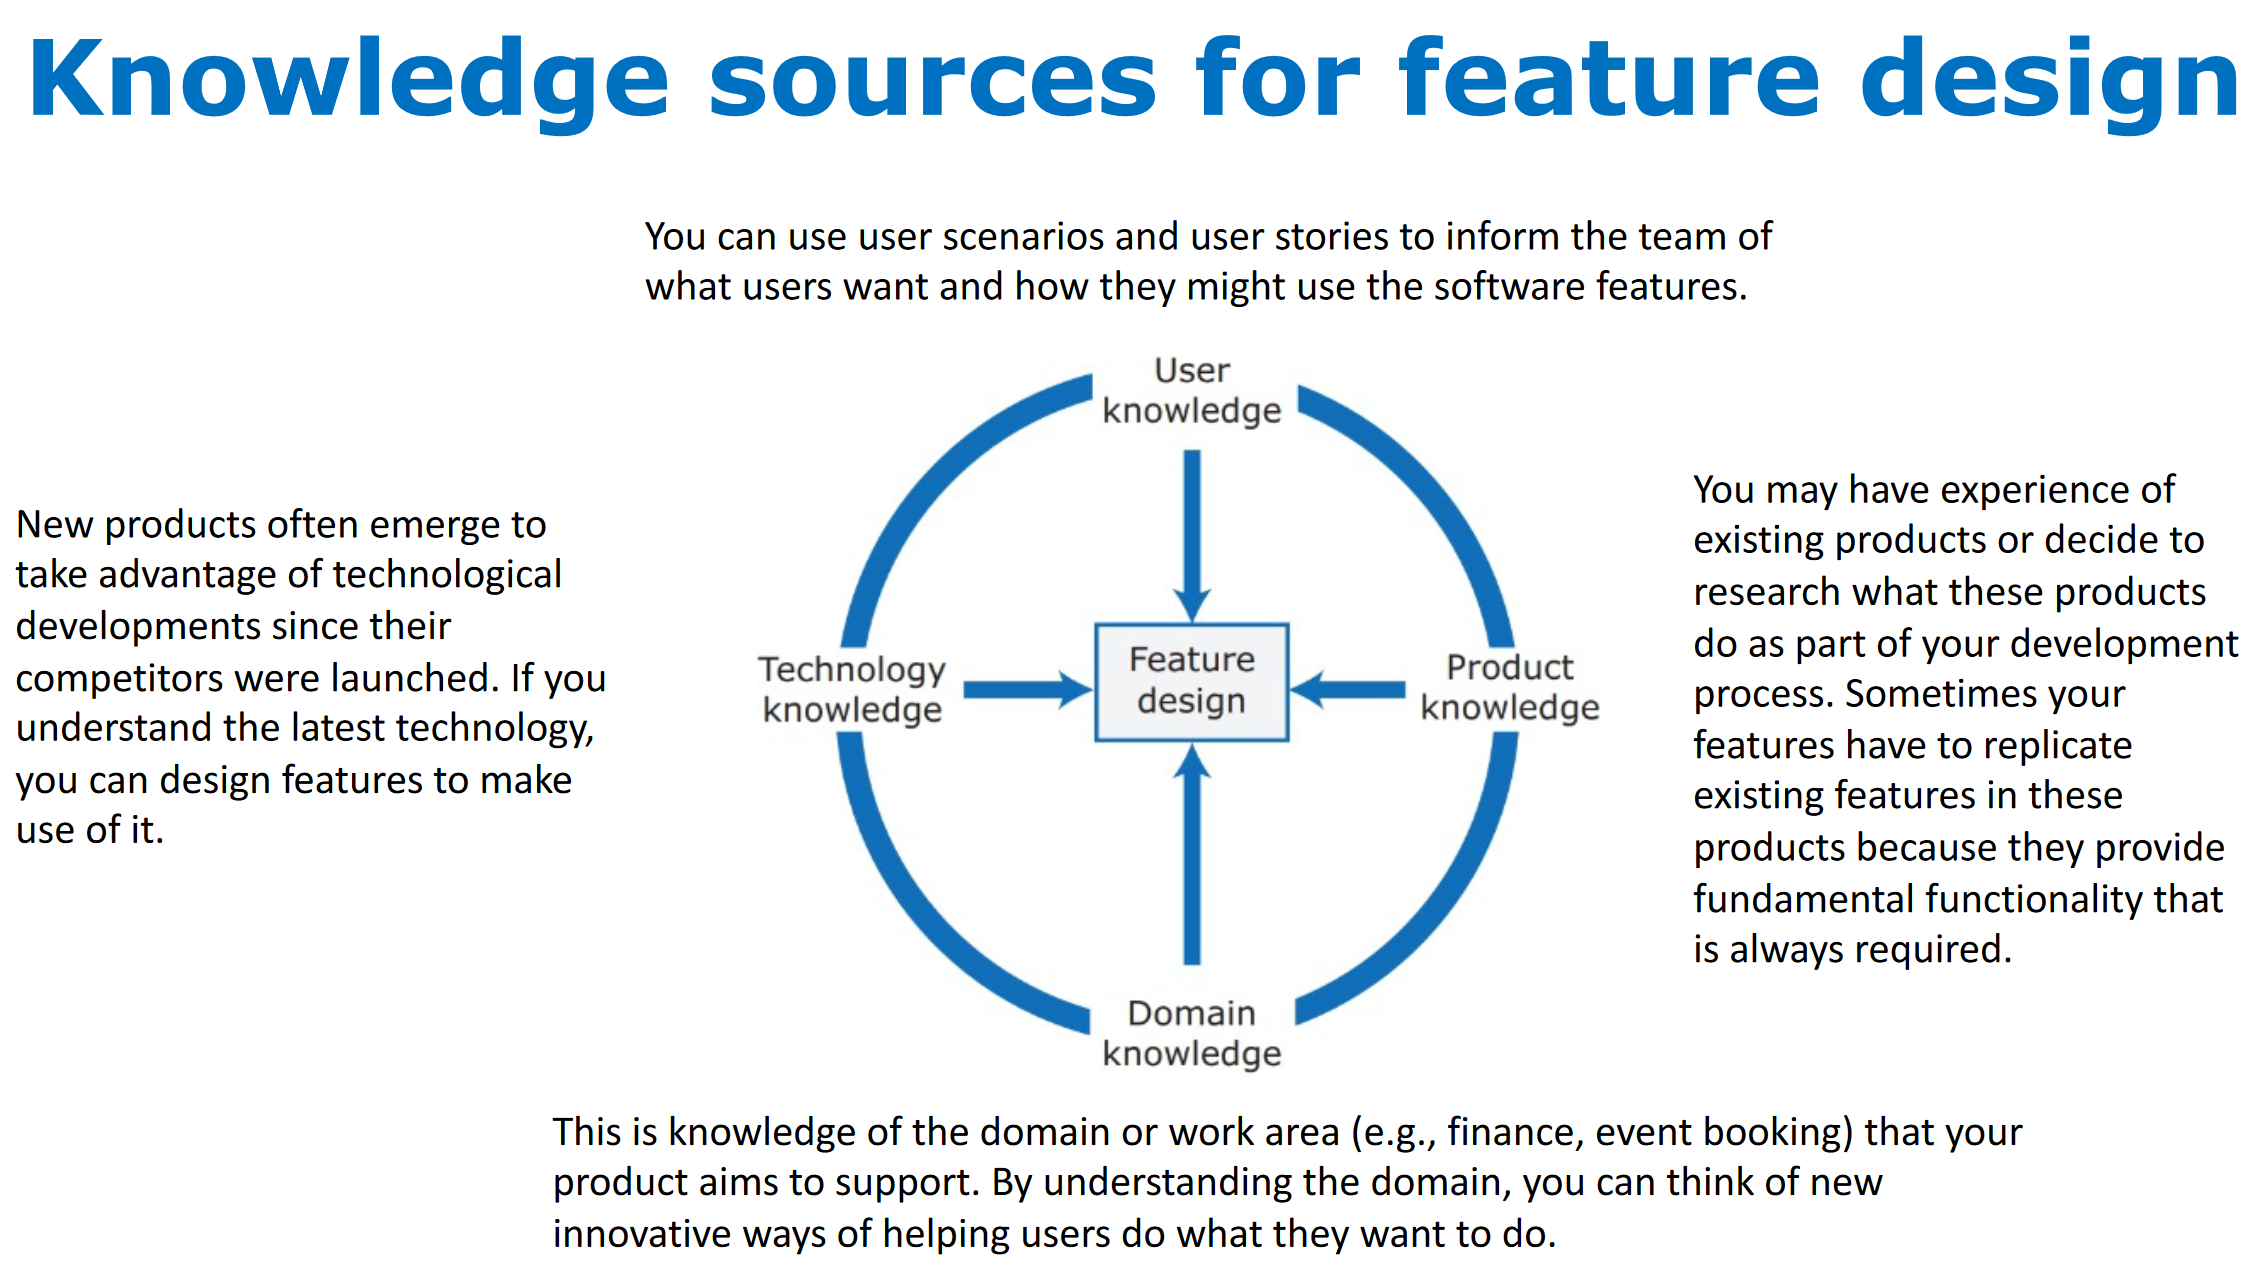
\includegraphics[width=0.9\textwidth]{images/feature_design.png}
    \caption{feature knowledge}
    \label{fig:feature_knowledge}
\end{figure}

To derive features from scenarios and user stories, the dev team should discuss these and start prototyping to demonstrate first novel and critical features.

\subsection{Feature Creep}
Number of product features grows as new potential users are envisaged.
To avoid this, 4 questions should be considered:
\begin{enumerate}
    \item Does this feature add something new or is it simply an alternative way of doing something already supported?
    \item Can this feature be implemented by extending an existing feat rather than adding a new one?
    \item Is this feat likely to be important and used by most software users?
    \item Does this feat provide general functionality or is it a very specific feat?
\end{enumerate}